% This is lnicst.tex the demonstration file of the LaTeX macro package for
% Lecture Notes of the Institute for Computer Sciences, Social-Informatics 
% and Telecommunications Engineering series from Springer-Verlag.
% It serves as a template for authors as well.
% version 1.0 for LaTeX2e
%
\documentclass[lnicst]{svmultln}
%
\usepackage{graphicx} % includegraphics
\usepackage{makeidx}  % allows for indexgeneration
\usepackage{url} %for url citing
\usepackage{caption}

% \makeindex          % be prepared for an author index
%
\begin{document}
%
\mainmatter              % start of the contribution
%
\title{Obfuscation with Turing Machine}
%
\titlerunning{Turing Machine Obfuscation}  % abbreviated title (for running head)
%                                     also used for the TOC unless
%                                     \toctitle is used
%
\author{Yan Wang\inst{1} \and Dinghao Wu,\inst{2}
Shuai Wang \and Pei Wang}
%
\authorrunning{Yan,Dinghao}   % abbreviated author list (for running head)
%
%%%% list of authors for the TOC (use if author list has to be modified)
\tocauthor{Ivar Ekeland, Roger Temam, Jeffrey Dean, David Grove,
Craig Chambers, Kim B. Bruce, Elisa Bertino}
%
\institute{Pennsylvania State University, State College,PA 16801, USA,\\
\email{ybw5084@ist.psu.edu} %\\ WWW home page:
%\texttt{http://users/\homedir iekeland/web/welcome.html}
% \and
% Universit\'{e} de Paris-Sud,
% Laboratoire d'Analyse Num\'{e}rique, B\^{a}timent 425,\\
% F-91405 Orsay Cedex, France}
}
\maketitle              
% typeset the title of the contribution
% \index{Ekeland, Ivar} % entries for the author index
% \index{Temam, Roger}  % of the whole volume
% \index{Dean, Jeffrey}

\begin{abstract}        % give a summary of your paper
Software security is a fundamental research domain in this threat emerging technology world. Control flow obfuscation one of important techniques to prevent hackers from understanding the program internal logic and leveraging software vulnerabilities to do damage. In this way, concealing important conditional branch logics are crucial for protecting software from being compromised. In this paper, we propose a novel control flow obfuscation method by leveraging the complexity of Turing machine. By entwining the original software programs with Turing machine execution, software control flow graph and call graph could be significantly complicated. We implemented an obfuscation tool named Turing machine obfuscator with LLVM. We evaluate the obfuscator by potency, resilience, stealth and cost respectively. Experiment results show that Turing machine obfuscator could obfuscate programs in stealth with good performance and robustness. 
%                         please supply keywords within your abstract
\keywords {software security, control flow obfuscation, Turing machine, LLVM}
\end{abstract}
%
\section{Introduction}
%
Obfuscation derives from intellectual property protection. The Internet brings us unprecedented convenience and threat of idea plagiarism and copyright infringement at the same time.  Concealing the algorithm of a software means a lot for the society especially for high-tech industry. Reverse engineering is often used by to recover source code from binaries to analyze software vulnerabilities or to steal software ideas or algorithms. Obfuscation is a technique to block or harden the process of reverse engineering.

Recently, Software security has become a bigger and bigger concern in research community because of infamous ransomware attack and severe vulnerability such as the recent ``Wanncry'' incidence and the OpenSSL heart bleeding bug.This incidences challenge the computer world greatly. Hackers endeavors to figure out venerabilities inside a software program. Knowing the software architecture and program logic like control flow graph is an indispensable prerequisite for hackers to analyze the original codes. With the help of some monitoring techniques hackers could even iterate all possible paths to try to restore all important branch information along the execution paths.\textit{Concolic testing} is an example which exploits symbolic execution given a certain input while it keeps changing input data until the code coverage proceed a threshhold\cite{Sen} as shown in Figure 1. It has been proved to work in restoring the branch information in the original source codes. Hence, a lot of research focus on preventing bad guys from figuring out the essential logic. Hiding important ``crossroad'' in a source program. Control flow obfuscation is one of these techniques. Control flow obfuscation aims at hiding conditional transfers and complicating the execution path within a source program. Through replacing or inserting extra control flow graph edges, the original software logic becomes harder or even impossible to trace. Previous research\cite{Ma} have proved the effectiveness of control flow obfuscation.

\begin{figure}
  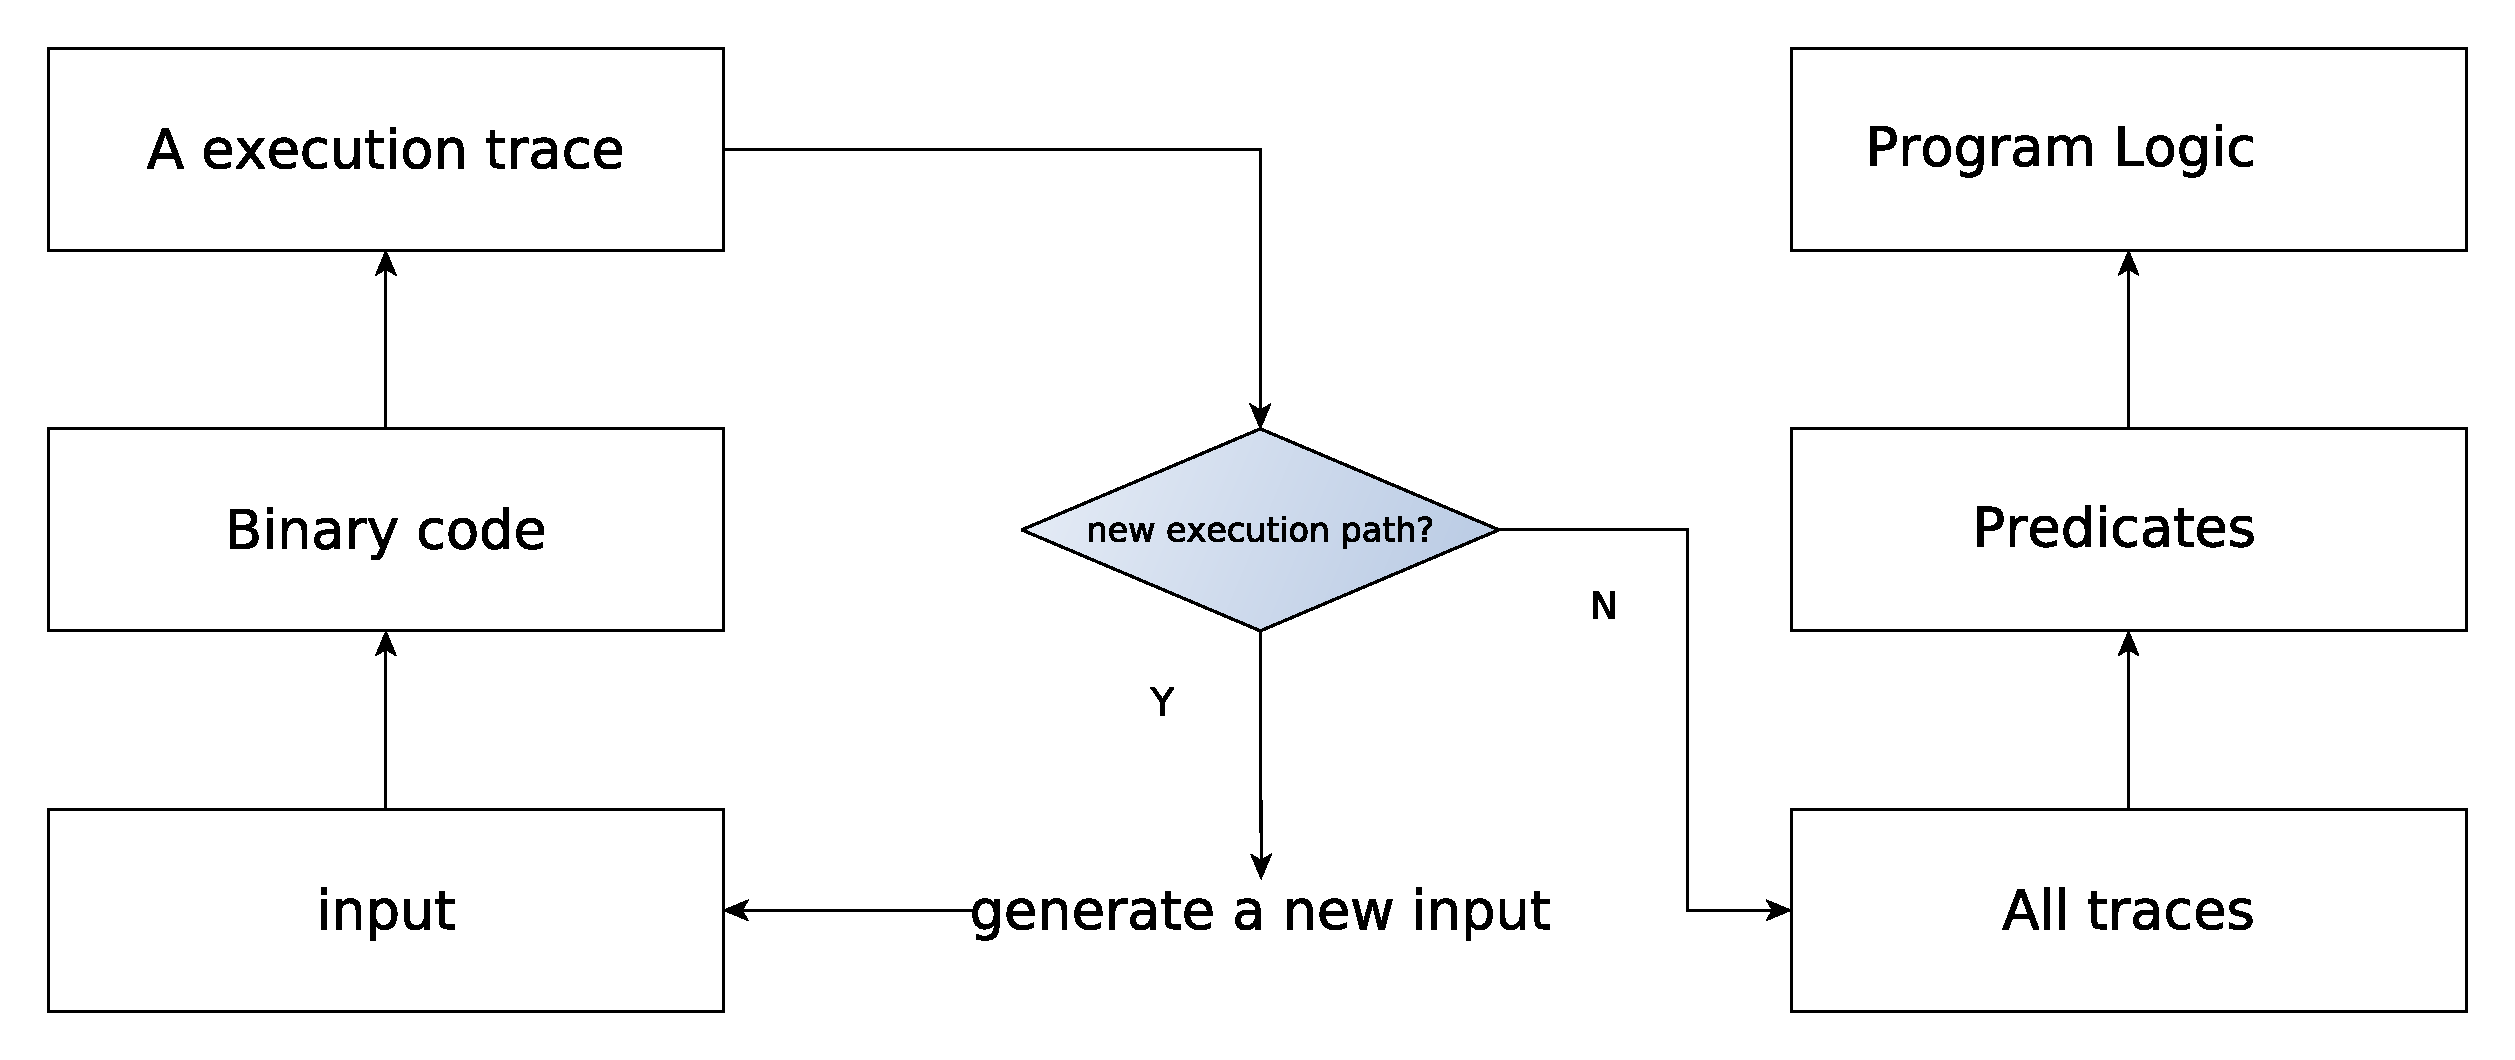
\includegraphics[width=0.9\linewidth]{reverse_engineering.eps}
  \caption{Reverse engineering with concolic testing}
  \label{Figure 1}
\end{figure}

In this paper, we propose a novel control flow obfuscation method with Turing machine embedded in the original program source codes. Turing machine is the essence of computation so it could calculate accurately all kinds of computer operation. In this way, important branch conditions in original source code could be replaced by a Turing machine execution which yields the very identical conditional value. Besides, a Turing machine behaves like a state machine so it contains a lot of branch condition checks in Turing machine transition table. In this whole process, sensitive branch information could be successfully hidden in Turing machine call graphs. In the meantime, Turing machine execution greatly introduces computational complexity to the target program so it is almost impossible to read the obfuscated programs to do reverse engineering. 

At the current stage, we only obfuscated conditional transfer instructions with integer operands. Utilizing LLVM, we could turn original program source codes into intermediate the representation(IR). Turing machine obfuscator takes over from IR and selects interested instruction candidates which would be redirected to semantic equivalent Turing machine execution. After iterating the call graph in the Turing machine ``black box'', the original call graph resumes from the  obfuscator interrupt and the whole program control flow graph is greatly expanded and complicated. Since LLVM is the implementation foundation, currently our proposed obfuscator could only be applied to C/C++ source programs. Inspired by previous works\cite{Collberg}, we evaluate our obfuscator from four dimensions which are potency, resilience, cost and stealth respectively. Results indicate that Turing machine obfuscator could effectively obfuscate target source codes with acceptable cost overhead.

This paper is organized as follows. Section 2 discusses related works on obfuscation, especially control flow obfuscation. Section 3 illustrate the idea and architecture of Turing machine obfuscator. Obfuscator implementation is discussed in section 4. Section 5 discusses the evaluation result of our proposed obfuscator. Finally, we conclude this paper in section 6.


%
\section{Related Works}
%
Generally speaking, reverse engineering is divided into static analysis such and dynamic analysis. To battle static reverse engineering, researchers usually focus on hardening disassembling and decompiling process. To combat the dynamic reverse engineering techniques such concolic testing, conditional transfer logic must be hidden from adversaries. Control flow obfuscation has been proved effective in previous works.

In \cite{Sharif}, the authors identified conditions that could trigger malware execution then using a hash function to transform the values which could launch malware. Afterward, correspondent conditional codes which would be run with the trigger value were encrypted with a key generated based on the instruction trigger value.
By this means the obfuscation analyzer could never get a chance to get the expected ``launching code'' consequently planted malware could never be executed. This technology works on certain fixed trigger value but not in scenarios that trigger values are intervals such as \textgreater \   and  \textless. This limitation narrows the applicable conditions greatly since a large volume of branch conditions are comparison operations. In addition, the encryption and decryption process in this methodology also introduce nonnegligible overhead.

In \cite{Popov}, the authors used signals(``traps'') to replace the control transfers unconditional instructions like ``jmp'' and ``call'' in order to confuse disassembly operation which is the first step of reverse engineering. Dummy control transfers and junk instructions were also inserted after signal replacements. This method seems to be effective in fooling disassemblers but it can't be applied in scenarios that conditional instruction logic needs to be protected from being figured out.

In \cite{Zhi}, the authors tried to cover branch information leveraging a remote trusted third party environment. The idea seemed to work while it not only introduced a great network overhead but also rely on trusted network accessibility which can't be guaranteed in reality. This drawback means this idea can't be applied in common obfuscation cases.

In \cite{Ma}, the authors took advantage of neural network to replace appropriate conditional instructions in source programs in order to achieve the goal of consealing conditional instruction logic thus dynamic analysis like concolic testing could never dig useful branch information. Although the idea looks promising and the results indicates the effectiveness of this methodology to some degree, fundamentally we don't believe neural networks solution is suitable for such scenarios. To the best of our knowledge,
neural networks work like a black box. It lacks the rigorous mathematical proof to illustrate a correct result must be generated given an input. Neural networks not only introduced complexity but also unpredictability to the original source programs. Trained models may behave very differently if given initial parameters with only some nuances, which means that it is also very hard to train an accurate enough model to simulate the conditional instruction. In addition, we noticed that neural networks consume too much memory in the evaluation experiments.

%
\section{Turing machine obfuscation}
%
In a computer program, conditional transfer instruction compares two operands and direct the following running path based on the comparison result. In theory, Turing machine has been proved to be able to simulate any algorithm and generate a corresponding correct answer. If a problem could be solved mathematically, it could definitely be solved by a Turing Machine. Taking advantage of Turing machine's powerful computational ability, complexity and mathematical correctness, we introduce Turing machine to the control flow obfuscation process. Through Turing machine execution, the identical boolean branching signal could be produced to guide further execution direction and the conditional logic is protected from being discovered. The intuitive methodology of Turing machine conditional branch transformation is shown in Figure 2.
\begin{figure}
 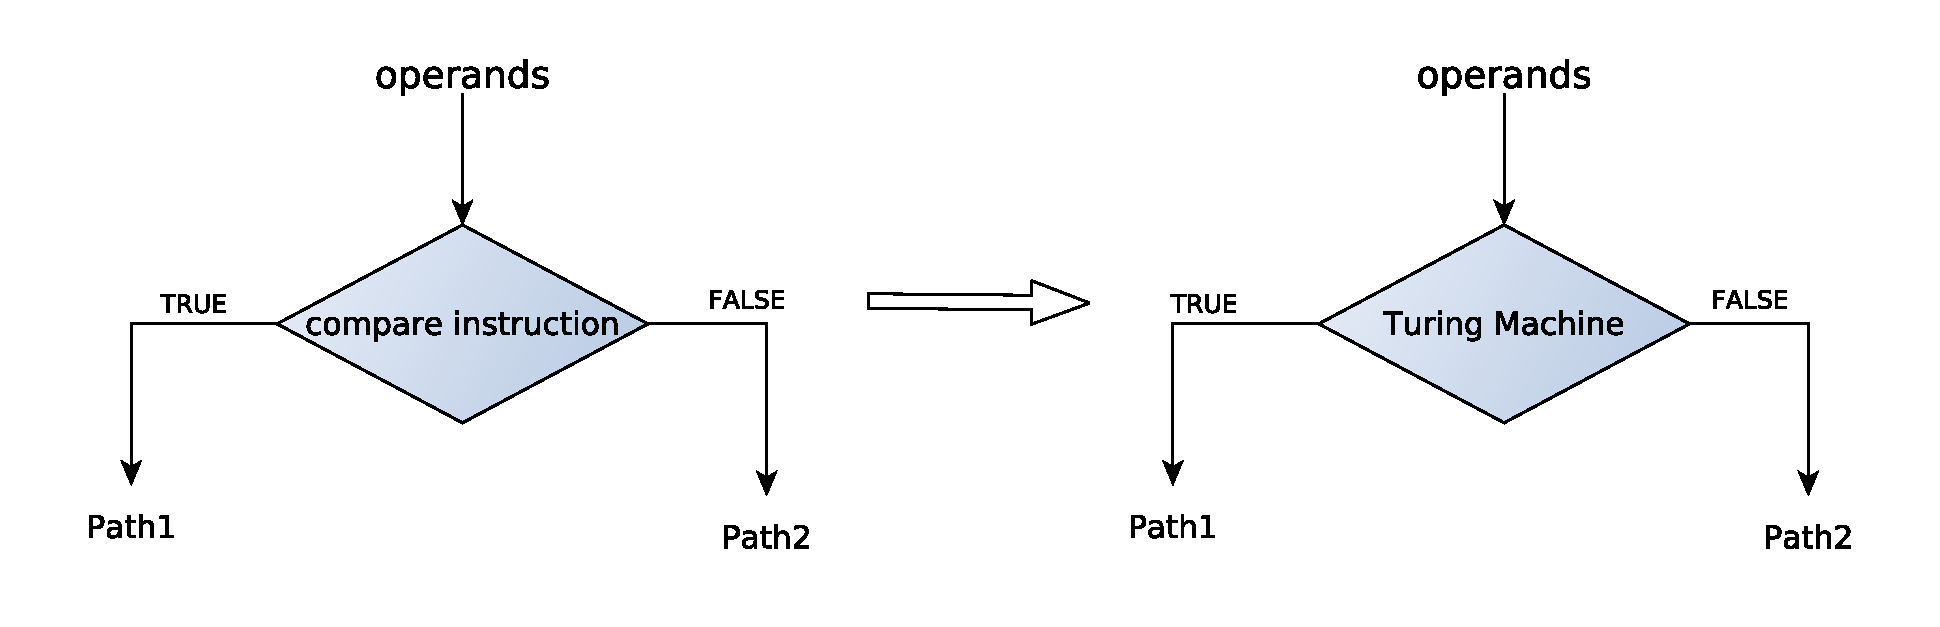
\includegraphics[width=\linewidth]{figure2.eps}
 \caption{Turing Machine Obfuscation Overview}
 \label{Figure 2}
\end{figure}

\subsection{Turing Machine}
Turing Machine is a mathematical model which could operate any computer program algorithm through reading and writing a infinite tape. Turing machine contains four components shown as Figure 4\cite{Turing}:
\begin{itemize}
  \item An infinite tape composed of cells. Each cell holds a symbol defined in the tape alphabet.
  \item A tape head which could conduct read, write, move left and move right operations.
  \item A state register used to record the state of the Turing machine. Turing machine states are finite.
  \item A transition table that consists of all the transition rules denoting how Turing machine transfer from one state to another.
\end{itemize}
\begin{figure}
 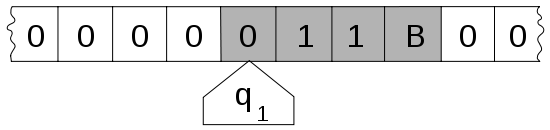
\includegraphics[width=0.9\linewidth]{Tm_tape.png}
 \caption{Turing Machine Components\cite{Turing}}
 \label{Figure 3}
\end{figure}
Formally a Turing machine could be represented by a 7 element tuple\cite{Turing}: \[ (Q, \Gamma, b, \Sigma, \delta, q_0, F) \] 
where:
\begin{itemize}
  %\renewcommand{\labelitemi}{$\star$}
  \item \(Q\) is finite state set
  \item \(\Gamma\) is finite tape symbol set named alphabet
  \item \(b\) is the tape blank symbol. \(b \in \Gamma\)
  \item \(\Sigma \subset \Gamma \)\textbackslash  \(\{b\}\) is the actual input symbol set without blank symbol
  \item \(\delta\) is the transition table composed of transition rules in form of \((Q\)\textbackslash \(F)\times\Gamma \rightarrow Q \times \Gamma \times \{L,R\}\) 
  \item \(q_0 \in Q \) is the initial state
  \item \(F\) is finite acceptable states set. \(F \subset Q\)
\end{itemize}

Given any program algorithm, there must be a corresponding Turing machine simulation. Since our Turing machine obfuscator concentrate on integer control transfer instruction replacement, Turing machine obfuscator contains transition tables which could do arithmatic operations like \(+, -, \times, \div\) and all compare operations like \(\leq,\geq , \neq\) \textit{etc.} Arithmatic operation result is displayed on tape when Turing machine reached the ``accept'' state. Compare operation result is 0 or 1 returned by Turing machine obfuscator.
\subsection{Universal Turing machine}
Although Turing machine could perform powerful and rigorous algorithm simulation, its inner logic is fixed and determined by the transition table. For instance, a Turing machine capable of doing adding operation could only simulate ``add'' operations. While in practical programs, control transfer could be any kinds of operation. Universal Turing machine is used to construction any kinds of Turing machine to simulate all necessary control flow transfer logic with different transition rules.

\section{Implementation}

\section{Evaluation}
Inspired by previous work\cite{Collberg}, we evaluated our Turing machine obfuscator based on four metrics which are \textit{potency}, \textit{resilience}, \textit{stealth} and \textit{cost} respectively. Potency weighs the complexity of a program in order to show how competent an obfuscator is. A good obfuscator also need to protect itself from being deobfuscated by tools. To measure how well an obfuscated program could withstand automatic deobfuscation techniques, metric resilience is introduced. Besides automated deobfuscators, a lot of reverse engineering works are conducted by hackers, obfuscated program should not be too different from the original one or it would be easy for adversaries to recognize. We used stealth to measure to how well a obfuscated program resembles the original one. Cost is naturally employed to measure computing overhead of a software program. Obfuscation would inevitably induce more overhead while the cost should be constricted to an acceptable level.

We choose two popular open source programs as target programs to verify the effectiveness of our Turing machine obfuscator: compress tool bzip2\cite{bzip2} and regular expression engine slre\cite{slre}. In Turing machine obfuscator, we filtered out all integer conditional transfer instruction as replacement candidates. Obfuscation level is an index which means the ratio between obfuscated instructions and all instruction candidates. In our experiments, we arbitrarily set it to 50\% which means half of all conditional transfer candidates are randomly chosen and obfuscated.
\subsection{Potency}
%
Control flow graph(CFG) and call  graph provide useful information about the general structure of a program so they are the traditional foundation for static software analysis. With the help of IDA Pro\cite{ida} which is a well-known commercial disassembler and debuger, we extracted CFG and call graph from original and obfuscated binaries. Through analyzing both graphs, we figured out basic block number, call graph edge number and control graph edge number. These static metrics are also used to indicate the complexity of a target program in previous work\cite{Chen}. Analysis result are shown in table 1. Comparing the metrics of source program and corresponding Turing machine obfuscated program, we found program complexity is strengthened in terms of each metric.


\begin{center}
 
 \begin{tabular}{|c | c | c | c|}
 \hline 
 Program & \# of CFG Edges & \# of Basic Blocks & \# of Function \\
 \hline
bzip2 & 4283 & 2837 & 78 \\ 
 \hline
obfuscated bzip2 & 4195 & 2828 & 134 \\
 \hline
regexp & 906 & 619 & 25 \\ 
 \hline
obfuscated regexp & 1122 & 773 & 43 \\
 \hline
\end{tabular}
\captionof{table}{}
\end{center}

Besides the traditional static evaluation, we refer to \cite{McCabe} and \cite{Woodward} to further quantify Turing machine obfuscated programs. The cyclomatic number and knot number were introduced in these works. Cyclomatic metric is defined as \[ Cyclomatic = E - N + 2 \] where E and N respectively represent the number of edges and the number of nodes in a CFG. Knot number means the amount of edge crossings in the CFG. These two metrics intuitively weighs how complicated a program is in terms of logic diversion number. Results in Table 2 show that both knot number and cyclomatic number increase after Turing machine obfuscation. Therefore, the potency of Turing machine obfuscator is proved.

\begin{center}
 \begin{tabular}{|c | c | c |} 
 \hline 
 Program & \# of Cyclomatic & \# of Knot \\
 \hline
bzip2 & 1448 & 11982  \\ 
 \hline
obfuscated bzip2 & 1369 & 5682  \\
 \hline
regexp & 289 & 478 \\ 
 \hline
obfuscated regexp & 351 & 1068 \\
 \hline
\end{tabular}
\captionof{table}{}
\end{center}

We pick 50\% as the obfuscation level to demonstrate the performance of Turing machine obfuscator while we also conducted experiments with other obfuscation level of 30\%, 80\% and 100\%. Figure 3 demonstrated that with a higher obfuscation level,  the number of call graph edge increases which indicates the obfuscated binary become more and more complicated. 
\begin{figure}
  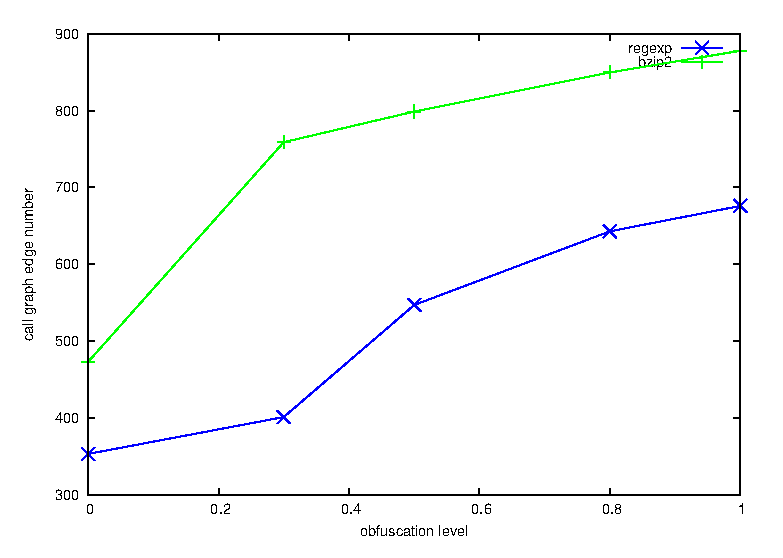
\includegraphics[width=0.9\linewidth]{cg.eps}
  \caption{Call graph Edge Number versus obfuscation level}
  \label{Figure 3}
\end{figure}

\subsection{Resilence}

\subsection{Stealth}
As mentioned in the beginning, software obfuscation technique should not only combat automated deobfuscation tools, but also manual deobfuscation methods. In the evaluation of stealth, authors of \cite{Trans} calculated the statistics of instruction distribution of both original and obfuscated programs to draw a comparison. If instruction distribution statistics of a obfuscated program is distinct from normal programs(e.g call or jmp instruction proportion is abnormally high), it would be a obvious indicator that denotes this program has been instrumented. We adopted this metric to evaluate our Turing obfuscator. Obfuscation level for stealth evaluation is set to 50\%.
\begin{figure}
  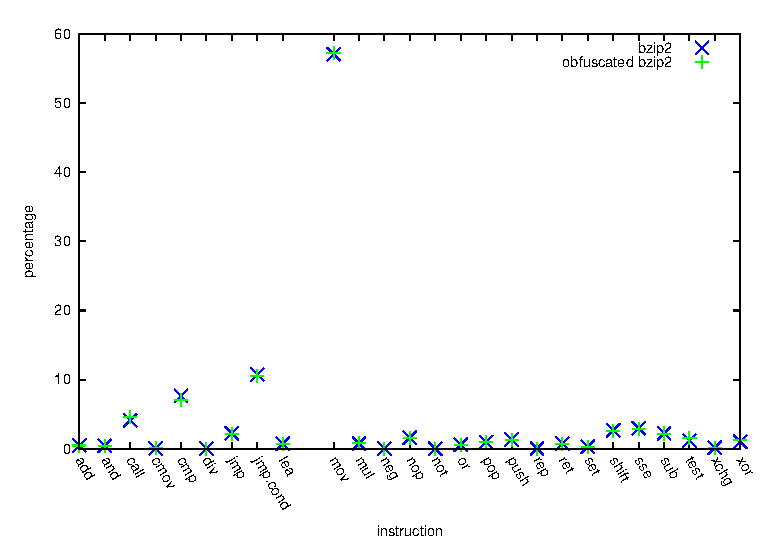
\includegraphics[width=0.9\linewidth]{st_bzip2.eps}
  \caption{bzip2 instruction distribution comparison}
  \label{Figure 4}
\end{figure}

\begin{figure}
  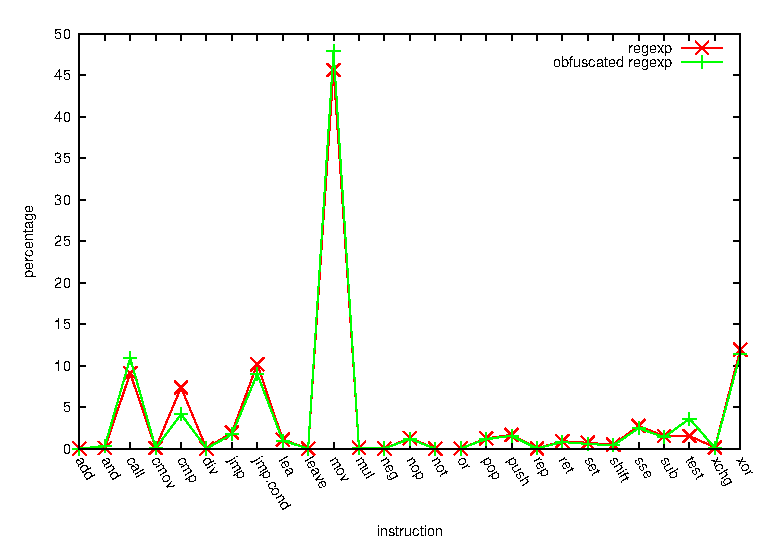
\includegraphics[width=0.9\linewidth]{st_regexp.eps}
  \caption{regexp instruction distribution comparison}
  \label{Figure 5}
\end{figure}
 We classified binary instructions into 27 different classes. Figure 4 and Figure 5 present the instruction distribution of the original and obfuscated version of target programs(bzip2 and regexp). Experiment results indicate that the instruction distribution after obfuscation is very close to the origin distribution. Given the fact that obfuscated binaries contain the same amount of extra instructions from Turing machine obfuscator, slre changed more than bzip2 because the former binary contains only 1391 lines of code and the later binary contains 8117 lines of code. Small instruction distribution variation indicated that our technique could obfuscate programs in stealth.

\subsection{Cost}
Software running cost is another important aspect in obfuscation evaluation. In most obfuscation research works, computing overhead increase is inevitable because obfuscation would induce extra instructions execution in one way or another. Measuring time cost is a simple and traditional way to evaluate to what extent an obfuscator induces execution overhead. In evaluation, source programs and obfuscated programs are run on a server with 2 Intel(R) Xeon(R) E5-2690 @ 2.90GHz processors and 125GB system memory.  Bzip2 compressed three different sample files and regular expession engine slre rans 149 test cases proviede by \cite{slre} in cost evaluation. We ran each program three times and recorded the average time cost as the final result.
\begin{figure}
  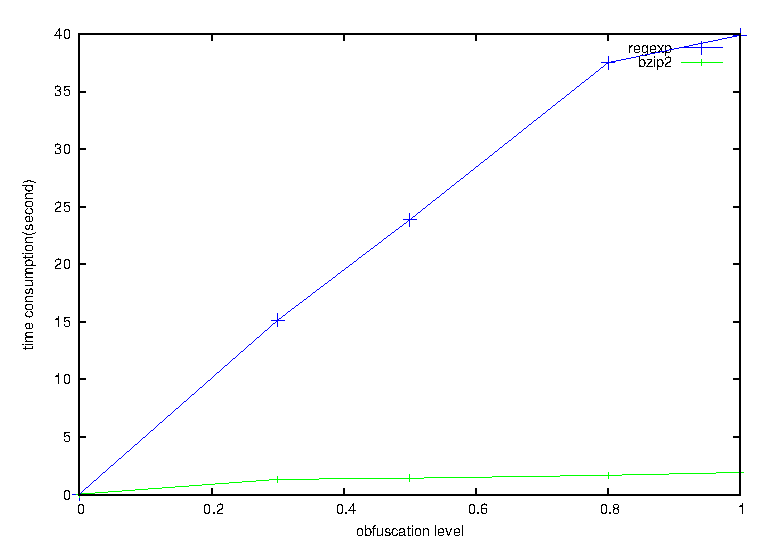
\includegraphics[width=0.9\linewidth]{cost.eps}
  \caption{Time cost versus obfuscation level}
  \label{Figure 6}
\end{figure}

Figure 6 demonstrates time cost monotonically increases with higher obfuscation levels for both target binaries. Obfuscated program takes more time to finish running as expected and we believe time cost is still confined to a reasonable level. We also noticed that there is a difference between slopes of the two curves. Turing obfuscator only randomly and statically obfuscates candidates instructions within a binary, so it does not ensure each chosen instruction candidate will be executed in the runtime. The curve slope difference probably result from the uncertainty of obfuscated instruction execution. In addition, the regexp program employs more recursive calls than the bzip2 program, this characteristic may also contribute to the rapid time cost increase of the regexp curve.

\section{Discussion}
\section{Conclusion}

%
% ---- Bibliography ----
%
\begin{thebibliography}{5}

\bibitem{Sen} Sen, Koushik, Darko Marinov, and Gul Agha. "CUTE: a concolic unit testing engine for C." ACM SIGSOFT Software Engineering Notes. Vol. 30. No. 5. ACM, 2005.

\bibitem{Ma} Ma, Haoyu, et al. "Control flow obfuscation using neural network to fight concolic testing." International Conference on Security and Privacy in Communication Systems. Springer International Publishing, 2014.

\bibitem{Trans} Wang, Pei, et al. "Translingual obfuscation." Security and Privacy (EuroS\&P), 2016 IEEE European Symposium on. IEEE, 2016.

\bibitem{Collberg} Collberg, Christian, Clark Thomborson, and Douglas Low. "Manufacturing cheap, resilient, and stealthy opaque constructs." Proceedings of the 25th ACM SIGPLAN-SIGACT symposium on Principles of programming languages. ACM, 1998.

\bibitem{Sharif} Sharif, Monirul I., et al. "Impeding Malware Analysis Using Conditional Code Obfuscation." NDSS. 2008.

\bibitem{Popov} Popov, Igor V., Saumya K. Debray, and Gregory R. Andrews. "Binary Obfuscation Using Signals." Usenix Security. 2007.

\bibitem{Zhi} Wang, Zhi, et al. "Branch obfuscation using code mobility and signal." Computer Software and Applications Conference Workshops (COMPSACW), 2012 IEEE 36th Annual. IEEE, 2012.

\bibitem{bzip2} \url{http://www.bzip.org/}

\bibitem{slre} \url{https://github.com/cesanta/slre}

\bibitem{Chen} Chen, Haibo, et al. "Control flow obfuscation with information flow tracking." Proceedings of the 42nd Annual IEEE/ACM International Symposium on Microarchitecture. ACM, 2009.

\bibitem{ida} \url{https://www.hex-rays.com/products/ida/}

\bibitem{McCabe} McCabe, Thomas J. "A complexity measure." IEEE Transactions on software Engineering 4 (1976): 308-320.

\bibitem{Woodward} Woodward, Martin R., Michael A. Hennell, and David Hedley. "A measure of control flow complexity in program text." IEEE Transactions on Software Engineering 1 (1979): 45-50.

\bibitem{Turing} \url{https://en.wikipedia.org/wiki/Turing_machine}
%%


\end{thebibliography}
%
\end{document}
